\documentclass[tikz,border=6pt]{standalone}
\usepackage{amsmath,amssymb,mathtools,physics,bm,nicefrac,wasysym}
\usepackage{xcolor}

\definecolor{colone}{RGB}{180,60,60}
\definecolor{coltwo}{RGB}{60,110,180}
\definecolor{colthree}{RGB}{60,140,80}

\definecolor{accent}{HTML}{A13D2C}
\definecolor{accent2}{HTML}{2B5F6B}
\definecolor{muted}{HTML}{5A564F}
\definecolor{panel}{HTML}{F8F6F0}
\definecolor{linecol}{HTML}{D8D2C4}
\definecolor{ink}{HTML}{1E1C1A}
\definecolor{astroblue}{HTML}{1B4F72}
\definecolor{astrodark}{HTML}{17202A}
\definecolor{sunyellow}{HTML}{E8A33D}

\usetikzlibrary{calc,arrows.meta,positioning,decorations.pathreplacing,decorations.markings,angles,quotes,shapes.geometric}
\usepackage{tikz-3dplot}

\newcommand{\vecr}{\vec r}
\newcommand{\vecL}{\vec L}
\newcommand{\vecA}{\vec A}
\newcommand{\vecf}{\vec f}
\newcommand{\vecF}{\vec F}
\newcommand{\vecp}{\vec p}
\newcommand{\avg}[1]{\left\langle #1\right\rangle}
\newcommand{\vecx}{\vec x}
\newcommand{\hatn}{\hat n}
\newcommand{\rhat}{\hat r}
\newcommand{\phihat}{\hat\phi}
\newcommand{\thetahat}{\hat\theta}
\newcommand{\note}[1]{\textcolor{blue!60!black}{\textit{[#1]}}}

% Astronomical acronyms
\newcommand{\LST}{\mathrm{LST}}
\newcommand{\GST}{\mathrm{GST}}
\newcommand{\GMST}{\mathrm{GMST}}
\newcommand{\GAST}{\mathrm{GAST}}
\newcommand{\LMST}{\mathrm{LMST}}
\newcommand{\LAST}{\mathrm{LAST}}
\newcommand{\UT}{\mathrm{UT}}
\newcommand{\UTC}{\mathrm{UTC}}
\newcommand{\TAI}{\mathrm{TAI}}
\newcommand{\TT}{\mathrm{TT}}
\newcommand{\TDB}{\mathrm{TDB}}
\newcommand{\JD}{\mathrm{JD}}
\newcommand{\MJD}{\mathrm{MJD}}
\newcommand{\EoT}{\mathrm{EoT}}
\newcommand{\SNR}{\mathrm{SNR}}
\newcommand{\RON}{\mathrm{RON}}

% Helper commands for specific diagrams
\newcommand{\midlinelabel}[3]{
    \node (midlabel) at ($ (#1)!.5!(#2) $) {#3};
    \draw[stealth-] (#1) --  (midlabel);
    \draw[-stealth] (midlabel) -- (#2);
}
\newcommand{\midlinelabell}[3]{
    \node[fill = white, inner sep = 0.2pt, outer sep=3pt] (midlabel) at ($ (#1)!.5!(#2) $) {#3};
    \draw[stealth-] (#1) --  (midlabel);
    \draw[-stealth] (midlabel) -- (#2);
}
\newcommand{\midlinelabelll}[3]{
    \node[fill = white, inner sep = 0.2pt, outer sep=3pt,scale=0.6] (midlabel) at ($ (#1)!.5!(#2) $) {#3};
    \draw[stealth-] (#1) --  (midlabel);
    \draw[-stealth] (midlabel) -- (#2);
}



\usepackage[T1]{fontenc}\usepackage{newpxtext,newpxmath}  % same fonts as the notes
\begin{document}
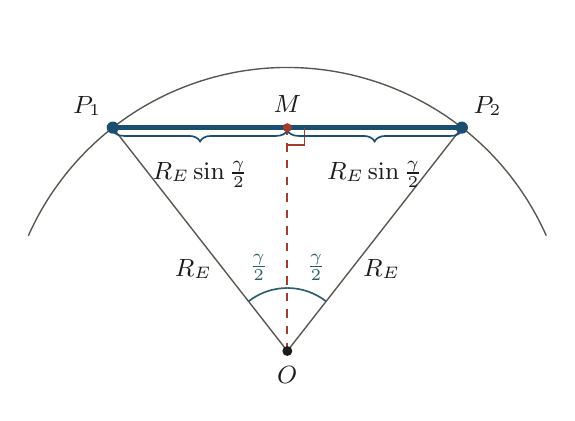
\begin{tikzpicture}[>=Stealth, lab/.style={font=\small, text=ink}]
  \def\RE{3.6}\def\g{76}
  \coordinate (O) at (0,0);
  \coordinate (A) at ({90+\g/2}:\RE);
  \coordinate (B) at ({90-\g/2}:\RE);
  \coordinate (M) at (90:{\RE*cos(\g/2)});
  \draw[muted, line width=0.5pt] ({90-\g/2-28}:\RE) arc ({90-\g/2-28}:{90+\g/2+28}:\RE);
  \draw[muted, line width=0.5pt] (O) -- (A);
  \draw[muted, line width=0.5pt] (O) -- (B);
  \draw[astroblue, line width=1.6pt] (A) -- (B);
  \draw[accent, dashed, line width=0.8pt] (O) -- (M);
  \draw[accent, line width=0.6pt] ($(M)+(0.22,0)$) -- ++(0,-0.22) -- ++(-0.22,0);
  % one brace per half, label inside the triangle
  \draw[decorate, decoration={brace, amplitude=4pt, mirror, raise=1pt}, astroblue, line width=0.6pt] (A) -- (M);
  \draw[decorate, decoration={brace, amplitude=4pt, mirror, raise=1pt}, astroblue, line width=0.6pt] (M) -- (B);
  \node[lab, below] at ($(A)!0.5!(M)+(0,-0.3)$) {$R_E\sin\frac{\gamma}{2}$};
  \node[lab, below] at ($(M)!0.5!(B)+(0,-0.3)$) {$R_E\sin\frac{\gamma}{2}$};
  % angles
  \draw[accent2, line width=0.6pt] ({90}:0.8) arc (90:{90+\g/2}:0.8);
  \draw[accent2, line width=0.6pt] ({90-\g/2}:0.8) arc ({90-\g/2}:90:0.8);
  \node[lab, text=accent2] at ({90+\g/4}:1.12) {$\frac{\gamma}{2}$};
  \node[lab, text=accent2] at ({90-\g/4}:1.12) {$\frac{\gamma}{2}$};
  \node[lab] at ($(O)!0.35!(A)+(-0.42,0.05)$) {$R_E$};
  \node[lab] at ($(O)!0.35!(B)+(0.42,0.05)$) {$R_E$};
  \fill[ink] (O) circle (1.8pt) node[lab, below=2pt] {$O$};
  \fill[astroblue] (A) circle (2.2pt) node[lab, above left=1pt] {$P_1$};
  \fill[astroblue] (B) circle (2.2pt) node[lab, above right=1pt] {$P_2$};
  \fill[accent] (M) circle (1.6pt) node[lab, above=2pt] {$M$};
\end{tikzpicture}
\end{document}
